% LTeX: language=en-US
\documentclass[a4paper,12pt,headinclude=true,headsepline,parskip=half,DIV=12]{scrartcl}

% Process this file using lualatex!
% > lualatex tutorial2.tex
% > biber lualatex2
% > lualatex tutorial2.tex

% font, style, etc.
\usepackage[automark]{scrlayer-scrpage}
\usepackage{csquotes}
\usepackage{xspace} % proper space after macros with 0 args

% mathematics
\usepackage{amsmath}
\usepackage{amssymb}
\usepackage{bm}
\usepackage{relsize}

% figures, tables, etc.
\usepackage{graphicx}
\usepackage{tikz}
\usepackage{pgf}
\usepackage{xcolor}
\usepackage{placeins} % -> floatbarrier

% Navigation
\usepackage{hyperref} %
\hypersetup{
    colorlinks = true, % false -> red box arround links (not very nice)
    linkcolor={blue!100!black},
    citecolor={blue!100!black},
    urlcolor={blue!100!black},
}

% others
\usepackage{siunitx}  % -> handling of units
\usepackage{acronym}
\usepackage[toc,page]{appendix}

% Code listings
\usepackage{luacode}
\usepackage{listings}
\lstset{
language=Python, 
backgroundcolor = \color{light-gray},
basicstyle=\scriptsize\sffamily,
stringstyle=\color{orange},
breaklines=true,
numberstyle=\tiny\color{gray},
keywordstyle=\bfseries\color{dark-blue}, % print keywords dark-blue
commentstyle=\color{dark-green}, % print comments dark-green
showstringspaces=false  % spacing between strings not showed
}

\luadirect{dofile("luainputlisting.lua")}
\newcommand*\luainputlisting[2]{
   \luadirect{print_code_part(\luastring{#1}, \luastring{#2})}
}
\newcommand*\luainputlistingline[2]{
   \luadirect{print_code_line(\luastring{#1}, \luastring{#2})}
}

% bibliography
\usepackage[backend=biber]{biblatex}
\addbibresource{literature.bib}

% manage glossaries
% Call makeglossaries tutorial1 on a command prompt after LaTeX compiling,
% the re-run LaTeX
% \usepackage{glossaries}
% \setacronymstyle{long-short}
% \makeglossaries
% \newacronym{ivp}{IVP}{initial value problem}
% \newacronym{ode}{ODE}{ordinary differential equation}

% theorems
\newtheorem{defi}{Definition}[section]

% define shortcuts
\newcommand{\ad}{\mathrm{ad}}
\renewcommand{\d}{\mathrm{d}} % d vor differential forms
\newcommand{\NV}{{\cal N}\,}
\newcommand{\rang}{\mathrm{rang}}
\newcommand{\im}{\mathrm{im}}
\newcommand{\spann}{\mathrm{span}}
\newcommand{\R}{\mathbb{R}} %  set of real numbers
\newcommand{\py}{Python\xspace}
\newcommand{\scipy}{SciPy\xspace}
\newcommand{\numpy}{NumPy\xspace}
\newcommand{\mpl}{Matplotlib\xspace}
\newcommand{\uu}{\mathbf{u}}
\newcommand{\f}{\mathbf{f}}
\newcommand{\x}{\mathbf{x}}
\newcommand{\y}{\mathbf{y}}
\newcommand{\z}{\mathbf{z}}
\newcommand{\xZero}{\mathbf{x}_0}
\newcommand{\yIZ}{y_{1A}}
\newcommand{\yIIZ}{y_{2A}}
\newcommand{\yIT}{y_{1B}}
\newcommand{\yIIT}{y_{2B}}
\newcommand{\diff}[2]{\frac{\text{d}#1}{\text{d}#2}}
\newcommand{\code}[1]{\lstinline[basicstyle=\normalsize\sffamily]|#1|}


% color definitions
\definecolor{light-gray}{gray}{0.95}
\definecolor{dark-blue}{rgb}{0, 0, 0.5}
\definecolor{dark-red}{rgb}{0.5, 0, 0}
\definecolor{dark-green}{rgb}{0, 0.5, 0}
\definecolor{gray}{rgb}{0.5, 0.5, 0.5}

% Avoid ugly indentations in footnotes.
\deffootnote[1em]{1em}{0em}{%
\textsuperscript{\thefootnotemark}%
}

\input{gevrey-package.tex}

% ----------------------------------------------------------------------------
\subject{\py for simulation, animation and control}
\title{Part 2: Tutorial for proper definition, computation and usage of reference trajectories}
\subtitle{Demonstration using the model of a kinematic vehicle}
\author{Max Pritzkoleit\thanks{Institute of Control Theory, Faculty of Electrical and Computer Engineering, Technische Universität Dresden, Germany} \and Jan Winkler\footnotemark[1]}
\date{\today}
% ----------------------------------------------------------------------------

% Headings
\setkomafont{pagehead}{\upshape}
\pagestyle{scrheadings}
\ihead{\leftmark}
\chead{}
\ohead{Page \pagemark}
\ifoot{}
\cfoot{Python Control Tutorial Part 2}
\ofoot{}

\begin{document}
\maketitle% create title

\tableofcontents

\newpage

\section{Introduction}
The goal of this tutorial is to teach the usage of the programming language \py as a tool for developing and simulating control systems. The following topics are covered:
\begin{itemize}
  \item Implementation of different trajectory generators in a \py class hierarchy,
  \item flatness based feedforward control
  \item flatness based feedback control.
\end{itemize}
Additionally, some aspects of object-oriented programming are covered as required to solve the presented problems.

Later in this tutorial the trajectory generators are used to design control strategies for the car model.

Please refer to the first part of this tutorial series addressing basic concepts for the simulation of dynamic systems if you are not familiar with this \cite{Tut1}. It is available on GitHub:
\begin{center}
  \href{https://github.com/TUD-RST/pytutorials}{https://github.com/TUD-RST/pytutorials}.
\end{center}
The book \cite{KnollPython21} is also recommended (in German only).



\section{Trajectories for smooth point-to-point transitions}
In control theory, a common task is to transfer a system quantity from an initial value $y^A$ at time $t_0$ to a new value $y^B$ at time $t_f$. The boundary conditions at $t_0$ and $t_f$ are a crucial part in the planning of such transfers. For example, if $y$ denotes a position coordinate and a simple trapezoidal interpolation in time between the two points $y^A$ and $y^B$ is used, the value of the acceleration $\ddot y$ at $t_0$ and $t_f$ would approach infinity. This cannot be fulfilled by any real system due to its inertia. That is why, when a point-to-point transition is planned, the derivative of the planned trajectory has to be smooth up to a certain degree. \autoref{fig:smoothtraj} shows an example of a "smooth" trajectory.

\begin{figure}[ht]
  \centering
  \includegraphics[scale=1]{img/state_transition.pdf}
  \caption{Smooth state transition of a quantity $y$ from $y^A$ to $y^B$ on the time interval $t_f - t_0$.}
  \label{fig:smoothtraj}
\end{figure}

Mathematically, the trajectory for a scalar quantity $y$ can be described by a function $f_y$ with $f_y : \mathbb{R} \to \mathbb{R}$. This function maps the domain of definition $\mathbb{R}$ onto the co-domain $\mathbb{R}$. This means that the function $f_y$ maps each time point $t \in \mathbb{R}$ in a certain way to a value $f_y(t) \in \mathbb{R}$. Usually this is denoted by $t \mapsto f_y(t)$. It is quite annoying to denote trajectories as $t \mapsto f_y(t)$ accompanied by the formal definition of a function $f_y$. Hence, as a shortcut, one simply writes $y = f_y(t)$ although -- literally speaking -- this notion just denotes the value of $f_y$ at time $t$. Especially in engineering science an even shorter notion is very common: One writes $y(t)$ instead of $t \mapsto f_y(t)$. This notion will be used in this tutorial, too.


\subsection{Polynomials} \label{sec:polynomials}
A simple way of defining a trajectory which realizes a smooth transfer between two values on the time interval $t_f - t_0$ and which is $d$ times continuously differentiable is the pieceewise definition of a function $y_d(t)$ as follows:
\begin{equation}
  y_d(t)=
  \begin{cases}
    y^A                                              & \textrm{if } t<t_0          \\[2ex]
    \mathlarger{\sum_{i=0}^{2d+1}}c_i\dfrac{t^i}{i!} & \textrm{if } t\in [t_0,t_f] \\[4ex]
    y^B                                              & \textrm{if } t>t_f
  \end{cases} \label{eq:TrajPoly}
\end{equation}
with a polynomial
\begin{equation}
  y_d(t)=\sum_{i=0}^{2d+1}c_i\frac{t^i}{i!} = c_0 + c_1 t + \frac{c_2}{2}t^2 + \frac{c_3}{6} t^3 + \ldots + \frac{c_{2d+1}}{(2d+1)!} t^{2d+1}
\end{equation}
of degree $2d+1$ which is evaluated on the interval $[t_0, t_1]$ only. Here, $2d+2$ boundary conditions for the determination of the coefficients $c_0, \ldots, c_{2d+1}$ need to be fulfilled at $t = t_0$ and $t = t_f$ ($d+1$ at each one).

For $t \in [t_0, t_f]$ $y_d(t)$ and its successive derivatives up to order $d$ can be written down in matrix form:
\begin{align}
  \label{eq:TMatrixFull}
  \underbrace{\begin{pmatrix}
                  y_d(t) \\ \dot{y}_d(t) \\ \vdots \\ y_d^{(d-1)}(t) \\ y_d^{(d)}(t)
                \end{pmatrix}}_{=:\mathbf{Y}_d(t) \in \R^{(d+1)}}
  =\underbrace{\begin{pmatrix}
                   1      & t      & \frac{t^2}{2!} &        & \hdots &        & \frac{t^{2d+1}}{(2d+1)!} \\[1ex]
                   0      & 1      & t              &        & \hdots &        & \frac{t^{2d}}{(2d)!}     \\[1ex]
                   0      & 0      & 1              &        & \hdots &        & \frac{t^{2d-1}}{(2d-1)!} \\[1ex]
                   \vdots &        & \ddots         & \ddots &        &        & \vdots                   \\[1ex]
                   0      & \hdots & \hdots         & 0      & 1      & \hdots & \frac{t^{d}}{(d)!}       \\[1ex]
                 \end{pmatrix}}_{=:\mathbf{T}(t) \;\in \; \R^{(d+1)\times (2d+2)}}
  \underbrace{
    \begin{pmatrix}
      c_0 \\ c_1 \\ \vdots \\ c_{2d-1}\\ c_{2d}\\ c_{2d+1}
    \end{pmatrix}}_{=:\mathbf{c}\in \R^{(2d+2)}}.
\end{align}
To calculate the parameter vector $\mathbf{c}$, the boundary conditions of the trajectory at $t_0$ and $t_f$ have to be defined up to degree $d$:
\begin{align*}
  \underbrace{\begin{pmatrix} y_d(t_0) \\ \dot{y}_d(t_0) \\ \vdots \\ y_d^{(d)}(t_0) \end{pmatrix}}_{:=\mathbf{Y}_d(t_0)}
   & \overset{!}{=}
  \underbrace{\begin{pmatrix} y^A \\ \dot{y}^A \\ \vdots \\ y^{(d)A}  \end{pmatrix}}_{:=\mathbf{Y}^A},
   &                &  &
  \underbrace{\begin{pmatrix} y_d(t_f) \\ \dot{y}_d(t_f) \\ \vdots \\ y_d^{(d)}(t_f) \end{pmatrix}}_{:=\mathbf{Y}_d(t_f)}
   & \overset{!}{=}
  \underbrace{\begin{pmatrix} y^B \\ \dot{y}^B \\ \vdots \\ y^{(d)B}  \end{pmatrix}}_{:=\mathbf{Y}^B}.
\end{align*}
This leads to a linear equation system:
\begin{align*}
  \begin{bmatrix}
    \mathbf{Y}_d(t_0) \\
    \mathbf{Y}_d(t_f)
  \end{bmatrix}
  =
  \begin{bmatrix}
    \mathbf{Y}^A \\
    \mathbf{Y}^B
  \end{bmatrix}
   & =
  \begin{bmatrix}
    \mathbf{T}(t_0) \\
    \mathbf{T}(t_f)
  \end{bmatrix}
  \mathbf{c}.
\end{align*}
Because $\begin{bmatrix}
    \mathbf{T}(t_0) \\
    \mathbf{T}(t_f)
  \end{bmatrix}$ is quadratic and not singular for $t_0\neq t_f$, this linear equation system can be solved explicitly:
\begin{align}
  \label{eq:2}
  \mathbf{c} & = \begin{bmatrix}
                   \mathbf{T}(t_0) \\
                   \mathbf{T}(t_f)
                 \end{bmatrix}^{-1}
  \begin{bmatrix}
    \mathbf{Y}^A \\
    \mathbf{Y}^B
  \end{bmatrix}.
\end{align}
Because the calculation of the inverse matrix is computationally expensive one is strongly advised to use a more efficient  linear equation system solver, like \code{linalg.solve()}  from \code{NumPy}, to solve for the vector $\mathbf{c}$.

$\mathbf{Y}_d(t)$ can be calculated in a closed form:
\begin{align}
  \label{eq:3}
  \mathbf{Y}_d(t)=\mathbf{T}(t)\mathbf{c} \quad t \in [t_0,t_f]
\end{align}
The full trajectory can be computed by evaluating \autoref{eq:TrajPoly}.

\paragraph{Remark:} Computational effort can be reduced if all derivates at $t_0$ and $t_f$ are zero (steady state transfer). Then, one can formulate \autoref{eq:TrajPoly} as
\begin{equation}
  y_d(t)=
  \begin{cases}
    y^A                                                      & \textrm{if } t < t_0         \\[2ex]
    \mathlarger{\sum_{i=0}^{2d+1}}c_i\dfrac{(t - t_0)^i}{i!} & \textrm{if } t \in [t_0,t_f] \\[4ex]
    y^B                                                      & \textrm{if } t > t_f
  \end{cases} \label{eq:TrajPolyAlt}
\end{equation}
Evaluating the boundary conditions at $t_0$ one observes $c_0 = y_d(t_0)$ and $c_1, \ldots, c_{d+1} = 0$. Then, the remaining coefficients $c_{d+2}, \ldots, c_{2d+2}$ can be computed from
\begin{align}
  \label{eq:PolyCoeffAlt}
  \begin{pmatrix}
    c_{d+2} \\ \vdots \\ c_{2d+2}
  \end{pmatrix}
  = \mathbf{T}_{d+1 \times d+1}^{-1}(t_f) \mathbf{Y}^B
\end{align}
where $\mathbf{T}_{d+1 \times d+1}$ is the quadratic lower right block matrix of \autoref{eq:TMatrixFull} evaluated at $t = t_f - t_0$.


\subsection{Polynomials using a prototype function}
A slightly different approach for a polynomial reference trajectory $y_d(t)$ is again a pieceewise-defined function:
\begin{align}
  \label{eq:PrototypeTraj}
  y_d(t) =
  \begin{cases}
    y^A                                                             & \textrm{if } t<t_0            \\
    y^A + (y^B-y^A)\varphi_\gamma\left(\frac{t-t_0}{t_f-t_0}\right) & \textrm{if } t \in [t_0, t_f] \\
    y^B                                                             & \textrm{if } t>t_f
  \end{cases}
\end{align}
with a prototype function $\tau \rightarrow \varphi_\gamma(\tau)$. The parameter $\gamma$ denotes  how often $\varphi_\gamma(\tau)$ is continuously differentiable. The prototype function meets  the following boundary conditions:
\begin{align}
  \varphi_\gamma(0)=0 \quad \varphi^{(j)}_\gamma(0)=0 \quad j = 1,...,\gamma, \\
  \varphi_\gamma(1)=1 \quad \varphi^{(j)}_\gamma(1)=0 \quad j = 1,...,\gamma,
\end{align}
and is given by
\begin{equation}
  \varphi_\gamma(\tau)= \frac{(2\gamma+1)!}{(\gamma!)^2} \sum_{k=0}^{\gamma} \binom{\gamma}{k} \frac{(-1)^k\tau^{\gamma+k+1}}{(\gamma+k+1)}
\end{equation}
with its $n$th derivative as
\begin{equation}
  \varphi_\gamma^{(n)}(\tau)= \frac{(2\gamma+1)!}{(\gamma!)^2} \sum_{k=0}^{\gamma} \left(\binom{\gamma}{k} \frac{(-1)^k\tau^{\gamma+k-n+1}}{(\gamma+k+1)}\prod_{i=1}^n(\gamma+k-i+2)\right).
\end{equation}

Note that the argument $\frac{t-t_0}{t_f-t_0}$ in \autoref{eq:PrototypeTraj} runs from 0 to 1 on the definition interval, indeed!.

The expression for the polynomial prototype is derived in \autoref{app:DerivePolyPrototype}.


\subsection{Gevrey functions} \label{sec:Gevrey}
Gevrey functions can come into play when you need to do trajectory planning for the control of infinite dimensional systems (e.g.\,systems with spatially distributed parameters). One type of such a function is provided by the trajectory generator class. Refer to \autoref{app:Gevery} for more details.



\section{Implementing trajectory generators in \py}
In order to automate the process of trajectory planning at first a trajectory generator base class is implemented. Then a new subclass for each new planning algorithm is created.

\textbf{\py Source code file: \code{TrajGen.py}}


\subsection{The trajectory generator base class}
A trajectory generator class realizing the smooth transfer from $y^A$ to $y^B$ on the interval $[t_0, t_f]$ should have the following attributes:
\begin{itemize}
  \item[] \code{YA} - vector of $y$ and it's derivatives up to order \code{d} at start time \code{t0}
  \item[] \code{YB} - vector of $y$ and it's derivatives up to order \code{d} at final time \code{tf}
  \item[] \code{t0} - start time of the point-to-point transition
  \item[] \code{tf} - final time of the point-to-point transition
  \item[] \code{d} - planned trajectory should be smooth up to the $d$-th derivative
\end{itemize}
The planned trajectory has to be evaluated at runtime, but the implementation of this feature should be defined in the specific subclass depending on the algorithm. Therefore, we define a base class \code{TrajGenBase} from which the several types of trajectory generator implementations need to be derived. By using an abstract base class method, we force a subclass of \code{TrajGenBase} to provide the methods \code{eval()} and \code{eval_vec()} for evaluation of the trajectory at a single point or for a series of points stored in an array-like container, respectively. For this purpose we need to import the \code{abc} module and need to derive the base class from the \code{ABC} class:
\luainputlisting{../sim/TrajGen.py}{TrajGen}
Note that any class derived from \code{TrajGenBase} needs to implement the methods decorated by \code{@abstractmethod}, otherwise a \code{TypeError} exception will be thrown when they are instantiated.

Note the special method \code{factorial} defined in the base class:
\luainputlisting{../sim/TrajGen.py}{FactorialFunc}
It is used for calculation of the factorial $x!$ of an integer $x$. Since it does not depend on any member variables it is defined as a class method. Class methods can be called without instantiation of a class, and they have only access to class attributes (defined outside \code{__init__})\footnote{In C++ and Java such methods are named \emph{static}.}. It is implemented here for didactic purposes only. Usually you would use \code{factorial} from the \code{math} or \code{scipy.special} module.


\subsection{The \emph{PolynomialTrajGen} subclass} \label{sec:polynomialTrajGen}
To implement the planning algorithm that was developed in \autoref{sec:polynomials}, a new class \code{PolynomialTrajGen} is created that inherits from the previously defined class \code{TrajGenBase}. All the attributes and methods of \code{TrajGenBase} are now also attributes and methods of \code{PolynomialTrajGen}. We define an additional attribute \code{c} holding the vector of coefficients of \autoref{eq:TrajPoly}:
\luainputlisting{../sim/TrajGen.py}{PolynomialTrajGen}
The built-in function \code{super()} tells the interpreter to call the constructor of the parent class of \code{PolynomialTrajGen}. As the code in \code{__init__} shows the coefficients are calculated. This is explained in the following.

To solve for the parameter vector $\mathbf{c}$, the matrix $\mathbf{T}(t)$ from \autoref{eq:TMatrixFull} is calculated and a method \code{t_matrix()} is therefore created:
\luainputlisting{../sim/TrajGen.py}{TMatrixFunDef}
Of course, this could be done more efficiently in a recursive way (try it!). Then, a method, that solves \autoref{eq:2} and returns the parameter vector $\mathbf{c}$ is needed:
\luainputlisting{../sim/TrajGen.py}{CoeffFunDef}
Finally a method \code{eval()} that implements \autoref{eq:3} is defined:
\luainputlisting{../sim/TrajGen.py}{PolynomialTrajGenEvalFunDef}
Furthermore, a second method \code{eval_vec()} is implemented, that can handle a time array as an input:
\luainputlisting{../sim/TrajGen.py}{PolynomialTrajGenEvalVecFunDef}
The polynomial trajectory generator is now successfully implemented and can be tested.

\textbf{Example:}

\textbf{\py source code file: \code{01_trajectory_planning.py}}

Suppose a trajectory from $y(t_0)=0$ to $y(t_f) = 1$ with $t_0=1s$ and $t_f = 2s$ has to be planned. The trajectory should be smoothly differentiable twice $(d=2)$. Therefore, the boundary conditions for the first and second derivative of $y$ have to be defined:
\begin{align*}
  \dot{y}(t_0)=0  &  &  & \dot{y}(t_f)=0  \\
  \ddot{y}(t_0)=0 &  &  & \ddot{y}(t_f)=0 \\
\end{align*}
The total time interval for the evaluation of the trajectory is $t\in[0s,3s]$.

At first the boundary conditions for $t=t_0$ and $t=t_f$ are set:
\luainputlisting{../sim/01_trajectory_planning.py}{ArrayDef}
After that the start and final time of the transition and the total time interval:
\luainputlisting{../sim/01_trajectory_planning.py}{TimeDef}
Then $d$ is set and a \code{PolynomialTrajGen} instance \code{yd} with the defined parameters is created.
\luainputlisting{../sim/01_trajectory_planning.py}{PolyTrajGenInstanciation}
The calculated parameters can be displayed
\luainputlistingline{../sim/01_trajectory_planning.py}{print("c}
and the generated trajectory at the defined total time interval can be evaluated
\luainputlistingline{../sim/01_trajectory_planning.py}{Y = yd}
At last, the results are plotted.
\luainputlisting{../sim/01_trajectory_planning.py}{CalcAndPlot}
\begin{figure}[ht]
  \centering
  \includegraphics[scale=0.9]{img/planned_trajectory.pdf}
\end{figure}


\subsection{The \emph{PrototypeTrajGen} subclass}

\textbf{\py Source code file: \code{TrajGen.py}}

The implementation can be found in the source code file. It is not detailed here since it is similar to the \code{PolynomialTrajGen}.



\section{Feedforward control design} \label{sec:ffcontrol}
\textbf{\py Source code file: \code{02_car_feedforward_control.py}}

Recapture the model of the car from tutorial 1 \cite{Tut1}, parameterized in time $t$:
\begin{subequations}
  \begin{align}
    \dot y_1    & = v \cos(\theta)            \\
    \dot y_2    & = v \sin(\theta)            \\
    \dot \theta & = \frac{v}{l}\tan(\varphi).
  \end{align}
\end{subequations}



\subsection{Re-parameterization of the model}
The model of the car has to be parameterized in arc length $s$ to take care of singularities that would appear in steady-state $(v=0)$.

The following can be assumed:
\begin{align*}
  \frac{\d}{\d t} = \frac{\d}{\d t}\frac{\d s}{\d s} = \frac{\d}{\d s}\frac{\d s}{\d t} = \frac{\d}{\d s}\dot s.
\end{align*}
Replacing $\frac{\d}{\d t}$ in the model equations leads to:
\begin{subequations}
  \begin{align}
    \frac{\d}{\d s}\dot s y_1    & = v \cos(\theta)            \\
    \frac{\d}{\d s}\dot s y_2    & = v \sin(\theta)            \\
    \frac{\d}{\d s}\dot s \theta & = \frac{v}{l}\tan(\varphi)
  \end{align}
\end{subequations}
\begin{align}
  v = |\dot{\bm{y}}| = \sqrt{\dot y_1^2+\dot y_2^2}.
\end{align}
This equation is parameterized in $s$:\footnote{Assuming $\dot s > 0$}
\begin{align}
  v = \sqrt{(\frac{\d}{\d s}\dot sy_1)^2+(\frac{\d}{\d s}\dot s y_2)^2}=\dot s \sqrt{(y_1^\prime)^2+(y_2^\prime)^2}.
\end{align}

If $s$ is the arc length, the Pythagorean theorem $ds^2 = dy_1^2 + dy_2^2$ leads to:
\begin{subequations}
  \begin{align}
    & 1 = \left(\frac{dy_1}{ds}\right)^2 + \left(\frac{dy_2}{ds}\right)^2 \\
    \Leftrightarrow \quad & 1 = \sqrt{(y_1^\prime)^2+(y_2^\prime)^2}.
  \end{align}
\end{subequations}
Therefore, $v=\dot s$.
The system parameterized in $s$ is given by:
\begin{subequations}
  \begin{align}
    y_1^\prime    & = \cos(\theta)              \\
    y_2^\prime    & = \sin(\theta)              \\
    \theta^\prime & = \frac{1}{l}\tan(\varphi).
  \end{align}
\end{subequations}



\subsection{Deriving feedforward control laws}
Goal: Drive the car in the $y_1$-$y_2$-plane from a point $(\yIZ, \yIIZ)$ to a point $(\yIT, \yIIT)$ in time $T=t_f-t_0$. The car should be in rest at the beginning and at the end of the process and the trajectory is defined by a sufficiently smooth function $f : \mathbb{R} \to \mathbb{R}$ with $y_2 = f(y_1)$. Note that $(y_1, y_2)$ is a flat output of the system.

\textbf{Step 1:} Calculate the dependency of the remaining system variables $\theta$ and $\varphi$ of the  length parameterized system on $(y_1, y_2)$:
\begin{align}
  \tan(\theta) & = \frac{y_2^\prime}{y_1^\prime} = \diff{y_2}{y_1} = f^\prime(y_1)\\
  (1 + \tan^2(\theta))\diff{\theta}{y_1} & = f^{\prime\prime}(y_1) \nonumber                                                                  \\
  \Leftrightarrow \quad \diff{\theta}{y_1} & = \frac{f^{\prime\prime}(y_1)}{1 + (f^\prime(y_1))^2} = \frac{\theta^\prime}{y_1^\prime}. \nonumber \\
  \intertext{With $(y_1^\prime)^2 + (y_2^\prime)^2 = 1 \, \Leftrightarrow \, y_1^\prime = 1/\sqrt{1 + (f^\prime(y_1))^2}$ one obtains:}
  \Leftrightarrow \quad \theta^\prime  & = \frac{f^{\prime\prime}(y_1)}{\left(1 + (f^\prime(y_1))^2\right)^{3/2}}\\
  \tan(\varphi)  & = l\theta^\prime = \frac{lf^{\prime\prime}(y_1)}{\left(1 + (f^\prime(y_1))^2\right)^{3/2}}.
\end{align}

Result: Depending on the planning $y_2 = f(y_1)$ the required steering angle can be calculated solely from $y_1$ and derivatives of $f$ w.r.t.~$y_1$ up to order 2. The planned trajectory has to fulfill the following boundary conditions:
\begin{align*}
  f(\yIZ) = \yIIZ  &  &  & f(\yIT) = \yIIT \\
  f^\prime(\yIZ) = \tan(\theta_A) &  &  & f^\prime(\yIT) = \tan(\theta_B) \\
  f^{\prime\prime}(\yIZ) = (1+\tan^2(\theta_A))\left(\frac{\frac{1}{l}\tan(\varphi_A)}{cos(\theta_A)}\right) &  &  &
  f^{\prime\prime}(\yIT) = (1+\tan^2(\theta_B))\left(\frac{\frac{1}{l}\tan(\varphi_B)}{cos(\theta_B)}\right).
\end{align*}
By always setting $\varphi_A=\varphi_B=0$, these conditions simplify to:
\begin{align*}
  f^{\prime\prime}(\yIZ) = 0 &  &  & f^{\prime\prime}(\yIT) = 0
\end{align*}
\textbf{Step 2:} Calculation of the required velocity $v$. Another function $g: \mathbb{R} \to \mathbb{R}$ is defined, with $y_1 = g(t)$ and $g(t_0) = \yIZ$, $\dot g(t_0) = 0$, $g(t_f) = \yIT$, $\dot g(t_f) = 0$.
\begin{align}
  v & = \sqrt{\dot y_1^2 + \dot y_2^2} = \dot y_1\sqrt{1 + (f^\prime(y_1))^2} = \dot g(t) \sqrt{1 + (f^\prime(g(t)))^2}
\end{align}

Hence, the overall, time parameterized feedforward control reads:
\begin{subequations}
  \label{eq:controllaw}
  \begin{align}
    v(t)       & = \dot g(t) \sqrt{1 + (f^\prime(g(t)))^2}                                                       \\
    \varphi(t) & = \arctan\left(\frac{lf^{\prime\prime}(g(t))}{\left(1 + (f^\prime(g(t)))^2\right)^{3/2}}\right)
  \end{align}
\end{subequations}
Or expressed in $s$:
\begin{subequations}
  \label{eq:controllaw_2}
  \begin{align}
    v(s)       & = \dot{s} \sqrt{y_2^{\prime2}+y_1^{\prime2}}                                                                                                                                                                              \\
    \varphi(s) & = \arctan\left(l \frac{y_2^{\prime\prime}y_1^\prime-y_1^{\prime\prime}y_2^\prime}{(y_1^{\prime2}+y_2^{\prime2})^{\frac{3}{2}}}\right) = \arctan\left(l (y_2^{\prime\prime}y_1^\prime-y_1^{\prime\prime}y_2^\prime)\right)
  \end{align}
\end{subequations}
If polynomials are chosen for the two functions $f$ and $g$ it has to be ensured that $f$ is of order 3 and $g$ of order 2 to make sure the control law is smooth. The resulting $f(g)$ is of order 5.


\subsection{Implementation}
For the implementation of the controller, the polynomial trajectory generator from \autoref{sec:polynomialTrajGen} is used.
At first all necessary simulation parameters are defined:
\luainputlisting{../sim/02_car_feedforward_control.py}{DefineSimPara}
We define a function which sets up the trajectory generator objects for trajectory generation:
\luainputlisting{../sim/02_car_feedforward_control.py}{DefineTrajGens}
Note, that we added type annotations here for the argument \code{sp} and the return value. This is optional. However, it is recommended since it improves static code analysis and IntelliSense features in your IDE. You need to import the typing module to use it for user defined types, lists and other complex data types. \href{https://www.python.org/dev/peps/pep-0483/}{More information about type hints...}

Within the right-hand side of the system differential equation the feedforward control law \eqref{eq:controllaw} needs to be evaluated. Hence, it needs to be implemented:
\luainputlisting{../sim/02_car_feedforward_control.py}{ControlLaw}
Now, the global trajectory objects can be instantiated and simulation can be executed as usual:
\luainputlisting{../sim/02_car_feedforward_control.py}{TrajSetupAndSim}
The results can be extracted by:
\luainputlistingline{../sim/02_car_feedforward_control.py}{x_traj = sol.y.T}
To get the control vector one has to evaluate \code{control()} with the simulated trajectory again:
\luainputlisting{../sim/02_car_feedforward_control.py}{ComputeControllerOutput}
Because \code{control()} works only for scalar time values, this has to be done in a \code{for}-loop. This is a bit annoying, but there is no alternative. It is impossible to store the control values when they are calculated within the right-hand side of the differential equation. The reason is that it is usually called by a variable step solver which evaluates it multiple times between the required time steps. 

Plotting the simulation results and the reference trajectories:
\luainputlisting{../sim/02_car_feedforward_control.py}{PlotResults}
Compared to the previous example \code{plot_data()} was adopted to also plot \code{x_ref}. 

\textbf{Exercise:} Modify the parameter $l$ in the control function, e.g.\,to 80\,\% of its real value. You will see that the feedforward control will drive the car to the wrong final position -- as expected, since no information about the real behavior of the car is fed back.


\subsubsection{Result} \label{subsec:result:ff}
As an example, the transition from $(0, 0, 0)$ to $(5, 5, 0)$, starting at $t=1s$ ending at $t=9s$ is shown in \autoref{fig:control_trajectory}. The whole simulation time interval goes from $t=0s$ to $t=10s$.
The animation shows the behavior of the car in the plane:
\begin{figure}[ht]
  \centering
  \includegraphics[scale=1]{img/plane_trajectory.pdf}
  \caption{Smooth state transition from $y^A$ to $y^B$ in the plane}
  \label{fig:plane_trajectory}
\end{figure}
\begin{figure}[ht]
  \centering
  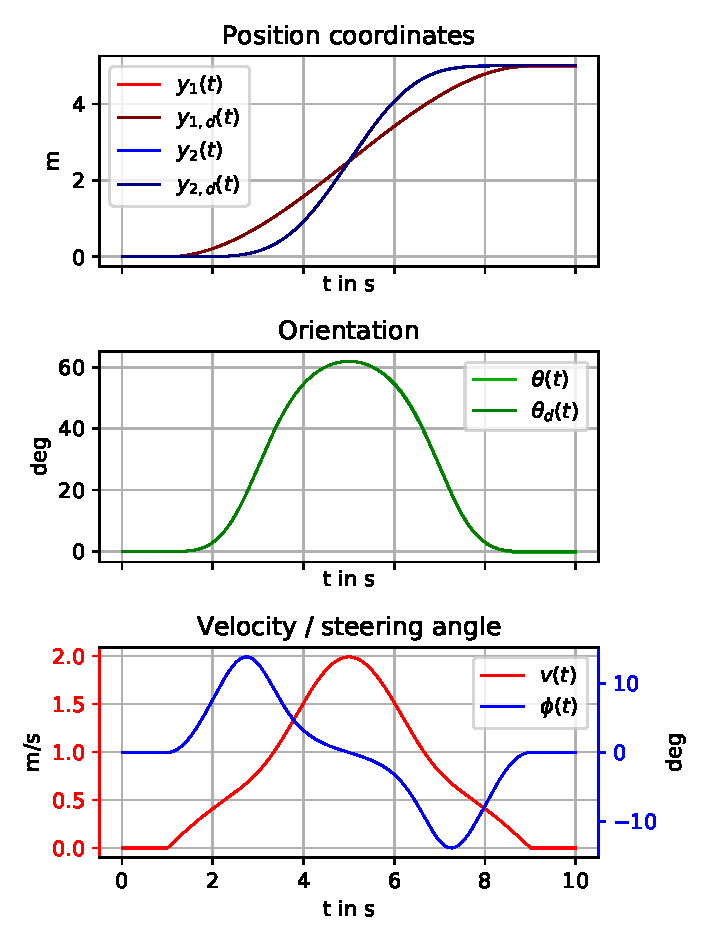
\includegraphics[scale=1]{img/control_trajectory.pdf}
  \caption{Feedforward control without model errors}
  \label{fig:control_trajectory}
\end{figure}
\clearpage



\section{Feedback control design} \label{sec:fbcontrol}

\textbf{Source code file: \code{03_car_feedback_control.py}}

In \autoref{sec:ffcontrol} the controller acts on the exact same system as it was designed for, but in the real world, model errors are inevitable, and a feedforward control is not sufficient. Assuming the length of the car in the controller $\tilde{l}$ differs from the real car length $l$ by a factor of $0.9$, the feedforward control of \autoref{subsec:result:ff} will show a bad performance.



\subsection{Deriving feedback control laws}
To account for model errors, a feedback controller has to be designed to fulfill the objective. This is done by a feedback linearization.
The linearization is done by introducing new inputs $w_1$ and $w_2$:
\begin{align}
  \label{eq:new_inputs}
  w_1 = y_1^\prime \qquad w_2 = y_2^{\prime\prime}.
\end{align}
This leads the linear system shown in \autoref{fig:linear_system}.
\begin{figure}[ht]
  \centering
  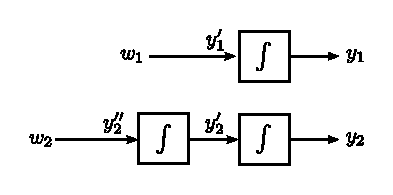
\includegraphics[scale=1]{img/linear_system.pdf}
  \caption{Block diagram of the linearized system}
  \label{fig:linear_system}
\end{figure}
The tracking error $e$ is defined as:
\begin{equation}
  \label{eq:error}
  e_i = y_i-y_{i,d} \qquad i = 1,2.
\end{equation}
A differential equation for the error term can be defined:
\begin{align}
  \label{eq:error_ode}
  0 = e_i^{\prime\prime}+k_{1i}e_i^{\prime}+k_{0i}e_i \qquad i = 1,2 \quad k_{0i},k_{1i} \in \R^+.
\end{align}
Substituting \autoref{eq:new_inputs} and \autoref{eq:error} in \autoref{eq:error_ode} leads to:
\begin{subequations}
  \begin{align}
    w_1 =  y_{1,d}^\prime - k_{01}(y_{1}-y_{1,d}) \\
    w_2 = y_{2,d}^{\prime\prime}  - k_{02}(y_{2}^\prime-y_{2,d}^\prime) - k_{02}(y_{2}-y_{2,d}).
  \end{align}
\end{subequations}
\begin{figure}[ht]
  \centering
  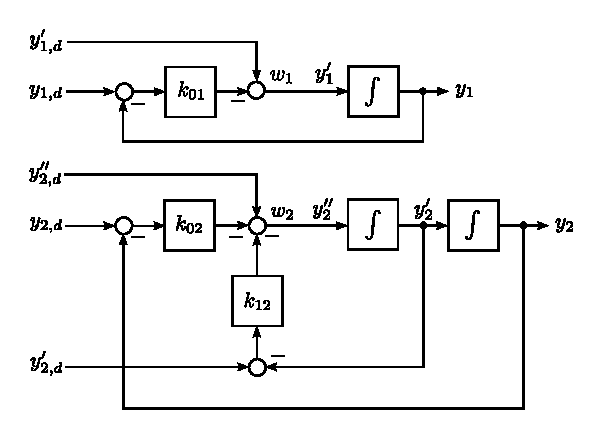
\includegraphics[scale=1]{img/linear_system_feedback.pdf}
  \caption{Block diagram of the feedback system}
  \label{fig:linear_system_feedback}
\end{figure}
These equations are substituted into \autoref{eq:controllaw_2} to obtain the feedback control law:
\begin{subequations}
  \begin{align}
    v(s)       & = \dot{s}_d\sqrt{w_1^2+y_2^{\prime 2}}\\
    \varphi(s) & = \arctan\left(l (w_2w_1-y_1^{\prime\prime}y_2^\prime)\right)
  \end{align}
\end{subequations}
where $\dot{s}_d$ is the desired velocity  and $y_1^{\prime\prime} = 0$.
To re-parametrize these control laws in time, the desired trajectories are expressed in $f$ and $g$:
\begin{subequations}
  \begin{align*}
    y_{1,d}        & = g(t)  &  &  & y_{2,d}             & = f(g(t))                                                  \\
    y_{1,d}^\prime & = \frac{1}{\sqrt{1+(f^{\prime }(g(t)))^2}} &  &  & y_{2,d}^\prime        & = \frac{f^{\prime }(g(t))}{\sqrt{1+(f^{\prime }(g(t)))^2}} \\
    \dot{s}_d      & = v_d(t) = \dot g(t) \sqrt{1 + (f^\prime(g(t)))^2} &  &  & y_{2,d}^{\prime\prime} & = \frac{f^{\prime \prime}(g(t))}{1+(f^{\prime }(g(t)))^2}.
  \end{align*}
\end{subequations}


\subsection{Implementation}
To implement the controller, at first the controller parameters are defined:
\luainputlisting{../sim/03_car_feedback_control.py}{DefineControllerPara}
The controller parameters have to be hand tuned and must be at least $>0$ for the system to be stable. In order to test the performance of the controller with respect to parameter uncertainties the real car length can be scaled, so a disturbed value is used in the control law.

The simulation parameter data class is extended by an attribute defining the real initial state of the car which might be different from what is planned:
\luainputlisting{../sim/03_car_feedback_control.py}{DefineSimPara}

Within the control law 
\luainputlisting{../sim/03_car_feedback_control.py}{ControlFunc}
the desired trajectories $f$ and $g$ are given in the objects \code{f_traj_gen} and \code{g_traj_gen} which are evaluated at the given time $t$ and then further processed:
\luainputlisting{../sim/03_car_feedback_control.py}{DefineRefTraj}
Afterwards $w_1$ and $w_2$ are set:
\luainputlisting{../sim/03_car_feedback_control.py}{CalcStabInputs}
In the final step, the control laws are calculated and returned from the function:
\luainputlisting{../sim/03_car_feedback_control.py}{ControlLaw}


\subsubsection{Result} \label{sec:result:fb}
The exercise from \autoref{subsec:result:ff} is repeated, but now using the feedback controller instead. As it can be seen in \autoref{fig:success_control} the control objective of following the planned trajectory succeeded, even with model errors.
\begin{figure}[ht]
  \centering
  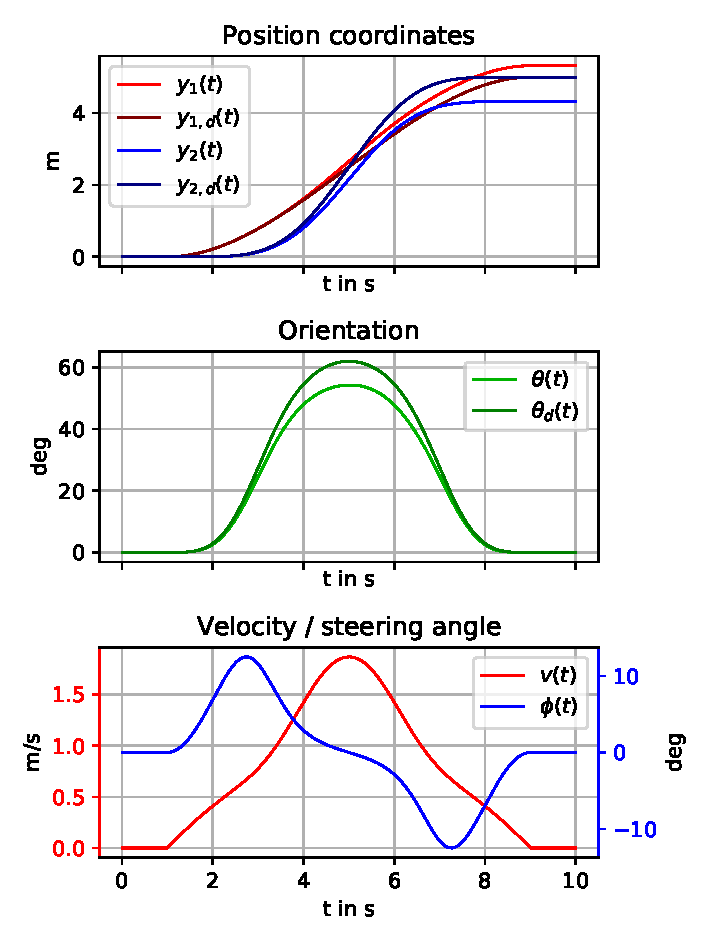
\includegraphics[scale=1]{img/failedcontrol.pdf}
  \caption{Feedforward control for $\tilde{l}=0.9l$. The car does not end up in the correct position.}
  \label{fig:failed_control}
\end{figure}
\begin{figure}[ht]
  \centering
  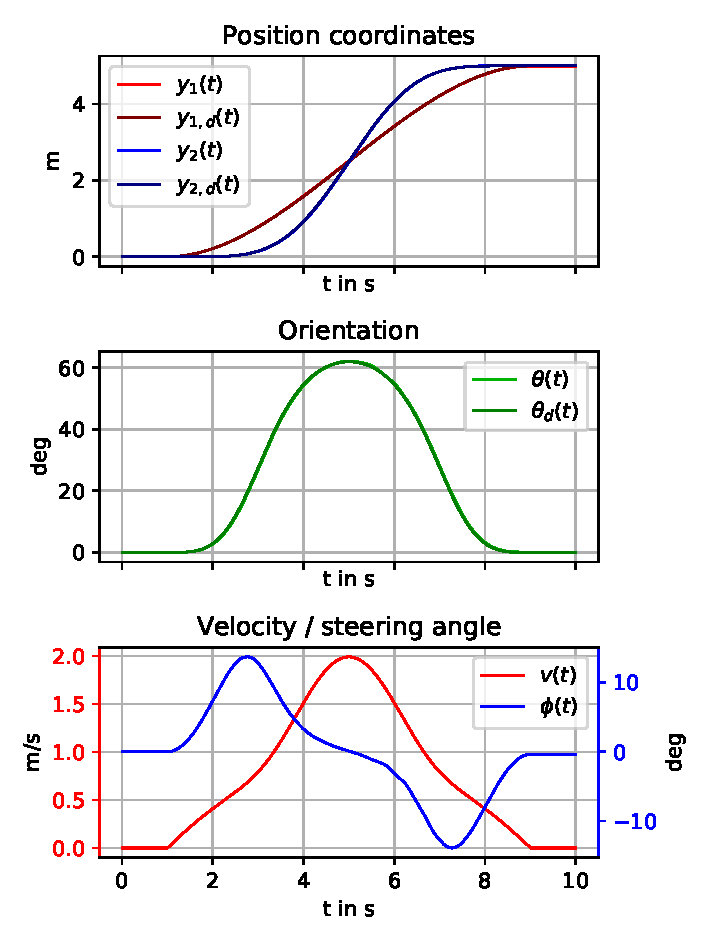
\includegraphics[scale=0.9]{img/successcontrol.pdf}
  \caption{Feedback control for $\tilde{l}=0.9l$. The car successfully reaches the planned final position.}
  \label{fig:success_control}
\end{figure}
\newpage
\clearpage



\begin{appendices}



  \section{The prototype polynomial} \label{app:DerivePolyPrototype}

  \begin{subequations}
    \label{eq:6}
    \begin{align}
      \varphi_\gamma(0)=0 \quad \varphi^{(j)}_\gamma(0)=0 \quad j = 1,...,\gamma \\
      \varphi_\gamma(1)=1 \quad \varphi^{(j)}_\gamma(1)=0 \quad j = 1,...,\gamma
    \end{align}
  \end{subequations}
  An approach for the derivative of $\varphi_\gamma(\tau)$, which meets the conditions \autoref{eq:6} is:
  \begin{align}
    \frac{\d \varphi_\gamma(\tau)}{\d \tau} = \alpha \frac{\tau^{\gamma}}{\gamma!}\frac{(1-\tau)^{\gamma}}{\gamma!}
  \end{align}
  Integration leads to:
  \begin{align}
    \varphi_\gamma(\tau) = \alpha \int_0^\tau\frac{\tilde{\tau}^{\gamma}}{\gamma!}\frac{(1-\tilde{\tau})^{\gamma}}{\gamma!} \d \tilde{\tau}
  \end{align}
  After $\gamma$ partial integrations we get:
  \begin{align*}
    \varphi_\gamma(\tau)= \frac{\alpha}{(\gamma!)^2} \sum_{k=0}^{\gamma} \binom{\gamma}{k} \frac{(-1)^k\tau^{\gamma+k+1}}{(\gamma+k+1)}
  \end{align*}
  To solve for the unknown $\alpha$, the  condition $\varphi_\gamma(1)\overset{!}{=}1$ is used:
  \begin{align*}
    \varphi_\gamma(1)=    & \frac{\alpha}{(\gamma!)^2} \sum_{k=0}^{\gamma} \binom{\gamma}{k} \frac{(-1)^k}{(\gamma+k+1)} \overset{!}{=} 1 \\
    \Leftrightarrow \quad & \alpha = (2\gamma+1)!
  \end{align*}
  Finally the prototype function is defined as:
  \begin{align}
    \varphi_\gamma(\tau)= \frac{(2\gamma+1)!}{(\gamma!)^2} \sum_{k=0}^{\gamma} \binom{\gamma}{k} \frac{(-1)^k\tau^{\gamma+k+1}}{(\gamma+k+1)}
  \end{align}
  and it's $n$-th derivative:
  \begin{align}
    \varphi_\gamma^{(n)}(\tau)= \frac{(2\gamma+1)!}{(\gamma!)^2} \sum_{k=0}^{\gamma} \left(\binom{\gamma}{k} \frac{(-1)^k\tau^{\gamma+k-n+1}}{(\gamma+k+1)}\prod_{i=1}^n(\gamma+k-i+2)\right)
  \end{align}
  In the last step the $n$-th derivative of \autoref{eq:PrototypeTraj} $(n=1,...,\gamma)$ is derived.
  \begin{align}
    y_d^{(n)}(t) = \begin{cases} 0                                                                                   & \textrm{if } t<t_0            \\
              \frac{(y^B-y^A)}{(t_f-t_0)^n}\varphi_\gamma^{(n)}\left(\frac{t-t_0}{t_f-t_0}\right) & \textrm{if } t \in [t_0, t_f] \\
              0                                                                                   & \textrm{if } t>t_f\end{cases}
  \end{align}




  \section{Trajectory generator based on a Gevrey function} \label{app:Gevery}
  It is sometimes necessary, that a planned trajectory is infinitely differentiable\footnote{For example in infinite dimensional systems control.}. A polynomial approach cannot be used in this case, because an infinite number of parameters is needed to construct such a polynomial. One approach to deal with this problem is to use Gevrey functions instead \cite{Rud03}.
  \begin{align*}
    y_d(t) = \begin{cases} y^A                                                             & \textrm{if } t<t_0            \\
              y^A + (y^B-y^A)\varphi_\sigma\left(\frac{t-t_0}{t_f-t_0}\right) & \textrm{if } t \in [t_0, t_f] \\
              y^B                                                             & \textrm{if } t>t_f\end{cases}
  \end{align*}
  
  
  
  \subsection{Definition}
  A function $\varphi:[0, T] \rightarrow \domR$ the derivatives of which are bounded on the interval $[0,T]$  by
  \begin{equation}\label{eq:gevrey:limit}
    \sup_{t \in [0,T]} \left| \varphi^{(k)}(t) \right| \leq m
    \frac{(k!)^{\alpha}}{\gamma^k}, \; \mbox{with} \;
    \alpha,\gamma,m,t   \in \domR, \quad k \geq 0
  \end{equation}
  is called a Gevrey function of order $\alpha$ on $[0, T]$.
  \begin{figure}[ht]
    \begin{center}
      \subfigure{\includegraphics[width=7cm]{img/gevrey0}}
      \subfigure{\includegraphics[width=7cm]{img/gevrey1}}
      \caption{Plot of function $\varphi_{\sigma,T}$  and its first derivative for different parameters.}
      \label{fig:gevrey}
    \end{center}
  \end{figure}
  Here we deal with the Gevrey function
  \begin{align}
    \varphi_\sigma\left(\tau\right) = \frac{1}{2}\left(1 + \tanh \left( \frac{2(2\tau-1)}{(4\tau(1-\tau))^\sigma}\right)\right)
  \end{align}
  which is based on the hyperbolic tangent. Some example plots of this function and its derivatives are given in
  \autoref{fig:gevrey}. The parameter $\sigma$ influences the steepness of the transition, for $\tau=\frac{t}{T}$, $T$ defines the length
  of the interval where the transition takes place. The order  $\alpha$ is given by $\alpha=1+1/\sigma$.
  %\begin{align}
  %\label{eq:gevrey:tanh:klasse} \alpha=1+1/\sigma.
  %\end{align}

  The function is not analytic in  $t=0 (\tau = 0)$ and $t=T (\tau = 1)$, all of its derivatives are zero in these points.
  
  
  
  \subsection{Efficient calculation of derivatives}
  \textbf{Problem:} Find an algorithm which calculates all derivatives of
  \begin{equation}\label{eq:defy}
    y:=\tanh\left(\frac{2(2\tau-1)}{(4\tau(1-\tau))^{\sigma}}\right)
  \end{equation}
  efficiently.

  \autoref{eq:defy} can be written as
  \begin{equation}\label{eq:shorty}
    y=\tanh(\dot{a}),\quad a=\frac{(4\tau(1-\tau))^{1-\sigma}}{2(\sigma-1)}.
  \end{equation}

  At first, we assume that all derivatives $a^{(n)},n \ge 0$ are known, and we show that an iteration formula can be given for $y^{(n)}$.

  Differentiating \autoref{eq:shorty} leads to
  \begin{equation}\label{eq:ydot}
    \dot{y}=\ddot{a}(1-\tanh^2(\dot{a}))=\ddot{a}(1-y^2).
  \end{equation}

  Introducing the new variable
  \begin{equation} \label{eq:defz}
    z:=(1-y^2),
  \end{equation}
  and differentiating \autoref{eq:ydot} $(n-1)$ times gives
  \begin{equation} \label{eq:formely_mit_z_und_a}
    y^{(n)}=\sum_{k=0}^{n-1}\tbinom
    {n-1}{k}a^{(k+2)}z^{(n-1-k)}.
  \end{equation}


  \textbf{Problem:} In \autoref{eq:formely_mit_z_und_a} derivatives of $z$ up to order $(n-1)$ are needed. These can be
  obtained by differentiating \autoref{eq:defz} $(n-1)$ times:
  \begin{equation*}
    %\label{eq:formelz}
    z^{(n-1)}=-\sum_{k=0}^{n-1}\tbinom
    {n-1}{k}y^{(k)}y^{(n-1-k)}.
  \end{equation*}


  Inspecting  \autoref{eq:formely_mit_z_und_a} one finds that an iteration formula for the derivatives of $a$ is missing. Using \autoref{eq:shorty} one gets
  \begin{equation*}
    \dot{a}=\frac{2(2\tau-1)}{(4\tau(1-\tau))^{-\sigma}}=\frac{(2\tau-1)(\sigma-1)}{\tau(1-\tau)}a.
  \end{equation*}

  Multiply this with ${\tau(1-\tau)}$ and differentiate it $(n-1)$ times:
  \begin{equation*}
    \sum_{k=0}^{n-1}\tbinom{n-1}{k} a^{(n-k)}\frac{d^k}{dt^k}(\tau(1-\tau))={(\sigma-1)}\sum_{k=0}^{n-1}\tbinom
    {n-1}{k} a^{(n-k-1)}\frac{d^k}{dt^k}(2\tau-1).
  \end{equation*}

  Solving for $a^{(n)}$ one gets
  \small
  \begin{align*}%\label{eq:formelalong}
    a^{(n)} & =\frac{1}{\tau(1-\tau)}\left((\sigma-1)\sum_{k=0}^{n-1}\tbinom{n-1}{k} a^{(n-k-1)}\frac{d^k}{dt^k}(2\tau-1)+\sum_{k=0}^{n-2}\tbinom{n-1}{k+1} a^{(n-k-1)}\frac{d^k}{dt^k}(2\tau-1)\right).
  \end{align*}
  \normalsize
  %%\begin{equation}
  %%a^{(2)}=\frac{4}{4\tau(1-\tau)}\left({\sigma}a^{(1)}(2\tau-1)+2(\sigma-1)a^{(0)}))\right)
  %%\end{equation}

  Note: The sums in the preceding equation have to be evaluated up to the second order only because higher derivatives of $(2\tau-1)$ vanish. The result reads
  \begin{equation*}
    a^{(n)}=\frac{1}{\tau(1-\tau)}\left((\sigma-2+n)(2\tau-1)a^{(n-1)}+(n-1)(2\sigma-4+n)a^{(n-2)}\right), n\ge 2.
  \end{equation*}
  
  
  
  \subsection{The \emph{GevreyTrajGen} subclass}
  The implementation can be found in the \textbf{\py source code file: \code{TrajGen.py}}.
\end{appendices}

\nocite{KnollPython21}


\printbibliography

\end{document}

%%% Local Variables:
%%% mode: latex
%%% TeX-master: t
%%% End:
